% !TeX root = ../paper.tex

\section{Entropic Affinities, Dimensionality Reduction and Optimal Transport}\label{sec:background}

% \begin{figure*}[t]
%     \begin{center}
%     \centerline{\includegraphics[width=\columnwidth]{figures/toy_kde.pdf}}
%     \caption{Kernel smoothing of a $1$-D signal corrupted with Gaussian noise using various affinity matrices. From left to right: row-normalized (stochastic) Gaussian kernel with constant bandwidth, DS Sinkhorn kernel with constant bandwidth (section \ref{sec:entropy_reg_OT}), entropic affinity (section \ref{sec:entropic_affinity}) and symmetric entropic affinity (section \ref{sec:sym_entropic_affinity}). Bandwidth and perplexity parameters are set to their optimal value using grid search, according to a mean squared error criterion, which optimal values are shown below each plot. Points'color represents the perplexity of the affinity matrix' associated row.}
%     \label{fig:toy_kde}
%     \end{center}
%     \vspace{-0.8cm}
% \end{figure*}

% This section covers all the necessary background material.



% $\mathcal{S}$ denotes the set of symmetric matrices. Finally we denote by $\mathcal{D} = \{\C \in \mathbb{R}_+^{n \times n} \:
% \text{s.t.} \: \C = \C^\top \: \text{and} \: C_{ij}=0 \iff i=j\}$ the set of admissible costs \ and $\mathcal{P} = \{\Pb \in \mathbb{R}_+^{n \times n} \:
% \text{s.t.} \: \Pb \bm{1} = \bm{1} \}$ the set of \nc{row-wise ?} stochastic matrices.

%In this section, we introduce the two key ingredients that we will link together in the next section, namely: entropic affinities (\cref{sec:entropic_affinities}) and symmetric entropic OT (\cref{sec:sEOT}) . 

%\subsection{Entropic Affinities and Applications to Dimensionality Reduction}\label{sec:entropic_affinities}

Given a dataset $\mathbf{X} \in \mathbb{R}^{n \times p}$ of $n$ samples in dimension $p$, most DR algorithms compute a representation of $\mathbf{X}$ in a lower-dimensional latent space $\mathbf{Z} \in \mathbb{R}^{n \times q}$ with $q \ll p$ that faithfully captures and represents pairwise dependencies between the samples (or rows) in $\X$. This is generally achieved by optimizing $\mathbf{Z}$ such that the corresponding affinity matrix matches another affinity matrix defined from $\X$. These affinities are constructed from a matrix $\mathbf{C} \in \R^{n \times n}$ that encodes a notion of ‘‘distance'' between the samples, \eg the squared Euclidean distance $C_{ij} = \|\mathbf{X}_{i:}-\mathbf{X}_{j:}\|_2^2$ or more generally any \emph{cost matrix} $\mathbf{C} \in \mathcal{D} := \{\Cb \in \mathbb{R}_+^{n \times n} : \Cb = \Cb^\top \text{and } C_{ij}=0 \iff i=j\}$. A commonly used option is the Gaussian affinity that is obtained by performing row-wise normalization of the kernel $\exp(-\Cb / \varepsilon)$, where $\varepsilon >0$ is the bandwidth parameter.

\paragraph{Entropic Affinities (EAs).} Another frequently used approach to generate affinities from $\mathbf{C} \in \mathcal{D}$ is to employ \emph{entropic affinities}  \cite{hinton2002stochastic}. The main idea is to consider \emph{adaptive} kernel bandwidths $(\varepsilon^\star_i)_{i \in \integ{n}}$ to capture finer structures in the data compared to constant bandwidths \cite{van2018recovering}. Indeed, EAs rescale distances to account for the varying density across regions of the dataset.

Given $\xi \in \integ{n-1}$, the goal of EAs is to build a Gaussian Markov chain transition matrix $\Pb^{\mathrm{e}}$ with prescribed entropy as
\begin{equation}
\begin{split}
    \forall i, \: &\forall j, \: P^{\mathrm{e}}_{ij} = \frac{\exp{(-C_{ij}/\varepsilon^\star_i)}}{\sum_\ell \exp{(-C_{i\ell}/\varepsilon^\star_i)}} \\
    &\text{with} \:\: \varepsilon^\star_i \in \mathbb{R}^*_+ \:\: \text{s.t.} \: \operatorname{H}(\Pb^{\mathrm{e}}_{i:}) = \log{\xi} + 1\,. \label{eq:entropic_affinity_pb}
\end{split}\tag{EA}
\end{equation}
The hyperparameter $\xi$, which is also known as \emph{perplexity}, can be interpreted as the effective number of neighbors for each data point \cite{vladymyrov2013entropic}. Indeed, a perplexity of $\xi$ means that each row of $\Pb^{\mathrm{e}}$ (which is a discrete probability since $\Pb^{\mathrm{e}}$ is row-wise stochastic) has the same entropy as a uniform distribution over $\xi$ neighbors. Therefore, it provides the practitioner with an interpretable parameter specifying which scale of dependencies the affinity matrix should faithfully capture. In practice, a root-finding algorithm is used to find the bandwidth parameters $(\varepsilon_i^\star)_{i \in \integ{n}}$ that satisfy the constraints \cite{vladymyrov2013entropic}. Hereafter, with a slight abuse of language, we call $e^{\operatorname{H}(\Pb_{i:})-1}$ the perplexity of the point $i$.

\paragraph{Dimension Reduction with SNE/t-SNE.} One of the main applications of EAs
is the DR algorithm \texttt{SNE} \cite{hinton2002stochastic}. We
denote by $\C_\X = \left(\|\X_{i:}-\X_{j:}\|_2^2\right)_{ij}$ and $\C_\Z =
\left(\|\Z_{i:}-\Z_{j:}\|_2^2\right)_{ij}$ the cost matrices derived from the
rows (\ie the samples) of $\X$ and $\Z$ respectively. \texttt{SNE} focuses on
minimizing in the latent coordinates $\Z \in \R^{n \times q}$ the objective
$\operatorname{KL}(\Pb^\mathrm{e} | \Qb_\Z)$ where $\Pb^\mathrm{e}$ solves
(\ref{eq:entropic_affinity_pb}) with cost $\C_\X$ and $[\Qb_\Z]_{ij} = \exp(-[\C_\Z]_{ij})/(\sum_{\ell}\exp(-[\C_\Z]_{i\ell}))$. In the seminal paper \citep{van2008visualizing}, a newer proposal for a \emph{symmetric} version was presented, which has since replaced \texttt{SNE} in practical applications. Given a symmetric
normalization for the similarities in latent space $[\widetilde{\Qb}_\Z]_{ij} = \exp(-[\C_\Z]_{ij})/\sum_{\ell,t}\exp(-[\C_\Z]_{\ell t})$ it consists in solving 
\begin{align}\label{symmetrization_tsne}
    \min_{\Z \in \R^{n \times q}} \: \operatorname{KL}(\overline{\Pb^{\mathrm{e}}} | \widetilde{\Qb}_\Z) \quad \text{where} \quad \overline{\Pb^{\mathrm{e}}} = \frac{1}{2}(\Pb^{\mathrm{e}} + \Pb^{\mathrm{e} \top}) \,.
\tag{Symmetric-SNE}
\end{align}
In other words, the affinity matrix $\overline{\Pb^{\mathrm{e}}}$ is the Euclidean projection of $\Pb^{\mathrm{e}}$ on the space of symmetric matrices $\mathcal{S}$: $\overline{\Pb^{\mathrm{e}}} = \operatorname{Proj}^{\ell_2}_{\mathcal{S}}(\Pb^{\mathrm{e}}) = \argmin_{\Pb \in \mathcal{S}}\| \Pb - \Pb^{\mathrm{e}} \|_2$ (see Appendix \ref{sec:sym_proj}). Instead of the Gaussian kernel, the popular extension t-SNE \citep{van2008visualizing} considers a different distribution in the latent space $[\widetilde{\Qb}_\Z]_{ij} = (1 + [\C_{\Z}]_{ij})^{-1}/\sum_{\ell,t}(1 +
[\C_{\Z}]_{\ell t})^{-1}$. In this formulation, $\widetilde{\Qb}_\Z$ is a joint
Student $t$-distribution that accounts for crowding effects: a relatively small
distance in a high-dimensional space can be accurately represented by a
significantly greater distance in the low-dimensional space.  

\noindent\begin{minipage}{0.45\linewidth}
Considering symmetric similarities is appealing since the proximity between two
points is inherently symmetric. Nonetheless, the Euclidean projection in
\eqref{symmetrization_tsne} \emph{does not preserve the construction of entropic
affinities}.  In particular, $\overline{\Pb^{\mathrm{e}}}$ is not stochastic in
general and $\operatorname{H}(\overline{\Pb_{i:}^{\mathrm{e}}}) \neq (\log{\xi} + 1)$ thus the entropy associated with each point is no longer controlled after symmetrization (see the bottom left plot of \cref{fig:coil}). This is
arguably one of the main drawbacks of the approach. By contrast, the
$\Pb^{\mathrm{se}}$ affinity that will be introduced in \cref{sec:sym_entropic_affinity} can
accurately set the entropy in each point to the desired value $\log \xi + 1$.  As shown in \cref{fig:coil} this leads to more faithful embeddings with higher silhouette scores when combined with the SNEkhorn algorithm (\cref{sec:DR_with_OT}).
\end{minipage}
\hspace{0.01\linewidth}
\begin{minipage}{0.53\linewidth}
\centering
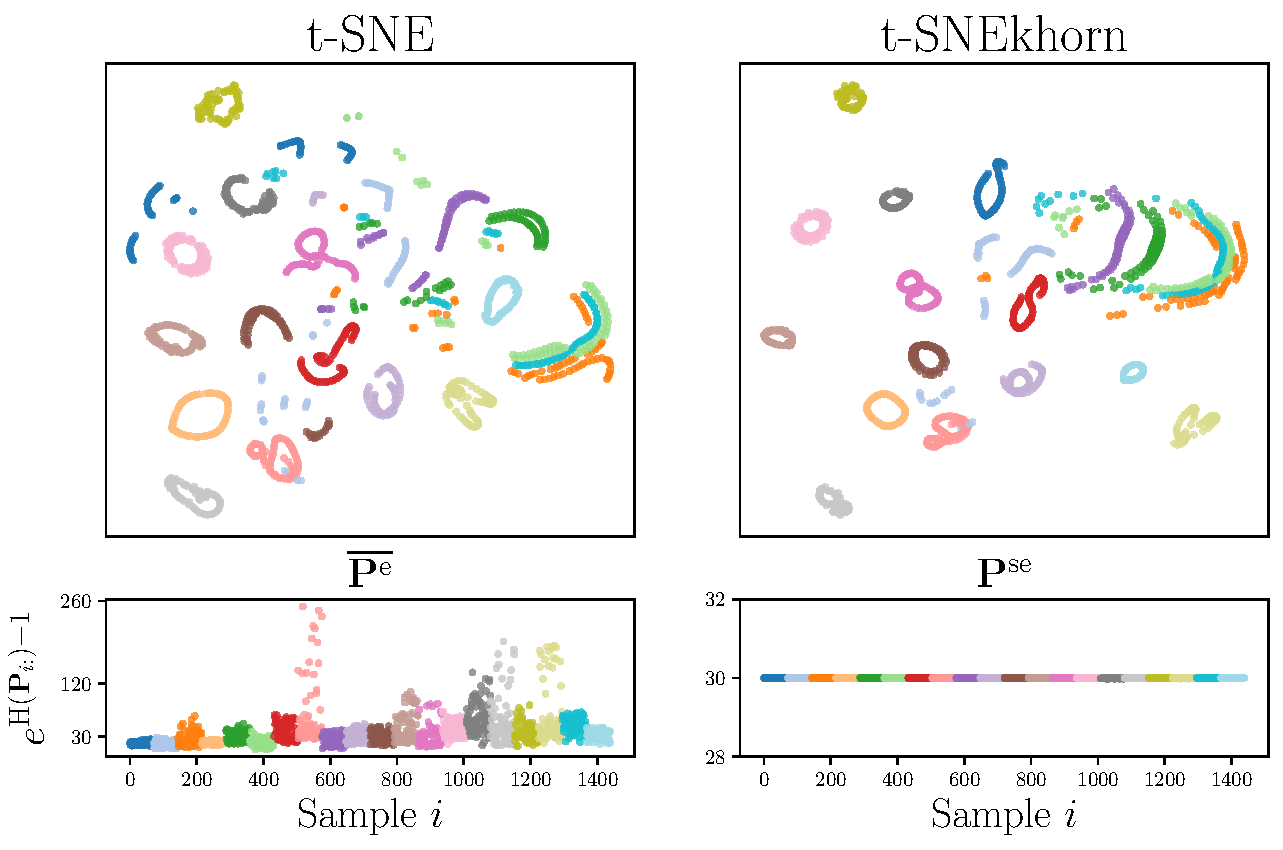
\includegraphics[width=\linewidth]{figures/SNEkhorn/fig_coil.pdf}
\captionof{figure}{Top: COIL \cite{nene1996columbia} embeddings with silhouette scores produced by Symmetric-SNE and SNEkhorn (our method introduced in  \cref{sec:DR_with_OT}) for $\xi=30$. Bottom: $e^{\operatorname{H}(\Pb_{i:})-1}$ (\emph{perplexity}) for each point $i$. \label{fig:coil}}
\end{minipage}

\paragraph{Symmetric Entropy-Constrained Optimal Transport.} Entropy-regularized
OT \citep{peyre2019computational} and its connection to affinity
matrices are crucial components in our solution. In the special case of uniform
marginals, and for $\nu > 0$, entropic OT computes the minimum of $\Pb
\mapsto \langle \Pb, \C \rangle -\nu \sum_{i} \operatorname{H}(\Pb_{i:})$
over the space of doubly stochastic matrices $\{\Pb \in \R_{+}^{n \times n} :
\Pb \bm{1} = \Pb^\top \bm{1} =\bm{1}\}$. The optimal solution is the
\emph{unique} doubly stochastic matrix $\Pb^{\mathrm{ds}}$ of the form $\Pb^{\mathrm{ds}}=\diag(\mathbf{u})\K
\diag(\mathbf{v})$ where $\K = \exp(-\C/\nu)$ is the Gibbs energy derived from
$\C$ and $\mathbf{u}, \mathbf{v}$ are positive vectors that can be found with
the celebrated Sinkhorn-Knopp’s algorithm \citep{cuturi2013sinkhorn,
sinkhorn1964relationship}. Interestingly, when the cost $\C$ is \emph{symmetric}
(\eg $\C \in \mathcal{D}$) we can take $\mathbf{u} = \mathbf{v}$ \cite[Section
5.2]{idel2016review} so that the unique optimal solution is itself symmetric and writes  
\begin{align}\label{eq:plan_sym_sinkhorn}
    \Pb^{\mathrm{ds}} = \exp \left((\mathbf{f} \oplus \mathbf{f} - \Cb) / \nu \right) \text{ where } \mathbf{f} \in \R^n \,.
\tag{DS}
\end{align}
In this case, by relying on convex duality as detailed in Appendix \ref{sec:proof_sinkhorn}, an equivalent formulation for the symmetric entropic OT problem is
% To define a DS affinity from $\X$ using OT, the somewhat counterintuitive idea is to transport the unit vector $\bm{1}$ to itself with transportation cost $\C_{\X}$. Note that, since $\C_{\X} \in \mathcal{D}$ is null on the diagonal, the unconstrained OT plan is trivially the identity matrix $\mathbf{I}_n$. To retrieve information about the samples' neighborhoods, the idea is to force the mass to spread outside the diagonal typically using constraints on the entropy of the OT plan.
% \begin{equation}
% \begin{split}
%     &\min_{\begin{smallmatrix} \Pb \in \R_{+}^{n \times n}: \ \Pb \bm{1} = \bm{1},  \Pb^\top \bm{1} = \bm{1}\end{smallmatrix}} \quad \langle \Pb, \C \rangle \quad -\nu \sum_{i} \operatorname{H}(\Pb_{i:}) 
%     %\text{s.t.} \quad \Pb \bm{1} = \bm{1}, \: \Pb = \Pb^\top \text{ and } \sum_i \operatorname{H}(\Pb_{i:}) \geq \eta \:,
% \end{split}
% \end{equation}
\begin{equation}
\tag{EOT}
\label{eq:entropy_constrained_OT}
\min_{\Pb \in \R_{+}^{n \times n}} \quad \langle \Pb, \Cb \rangle \quad \text{s.t.} \quad \Pb \bm{1} = \bm{1}, \: \Pb = \Pb^\top \text{ and } \sum_i \operatorname{H}(\Pb_{i:}) \geq \eta \:,
\end{equation}
where $0 \leq \eta \leq n (\log n + 1)$ is a constraint on the global entropy $\sum_i \operatorname{H}(\Pb_{i:})$ of the OT plan $\Pb$ which happens to be saturated at optimum (Appendix \ref{sec:proof_sinkhorn}). This constrained formulation of symmetric entropic OT will provide new insights into entropic affinities, as detailed in the next sections.

% \begin{remark}\label{rem:sink_proj}
%     For a set $\mathcal{E}$, we denote $\operatorname{Proj}^{\operatorname{\KL}}_{\mathcal{E}}(\K) = \argmin_{\Pb \in \mathcal{E}}\KL(\Pb | \K)$ the projection on $\mathcal{E}$ under the $\KL$ geometry. Then \cite{benamou2015iterative} shows that $\Pb^s = \operatorname{Proj}^{\operatorname{\KL}}_{\mathcal{P} \cap \mathcal{S}}(\K)$ is another way of characterizing the solution of problem (\ref{eq:entropy_constrained_OT}), which thus consists in projecting a Gaussian kernel onto the set of doubly stochastic matrices under the $\KL$ geometry. As shown in \cite{Zass}, finding this closest doubly stochastic matrix can be linked to solving a relaxed cluster assignment problem. \titouan{vraiment pas sûr de 'intéret de cette remarque ici, + c'est pas vraiment proj sur P et S, c'est proj sur P, S et entropie globale geq than $\eta$}
%     %In this framework, the KL is linked to normalized cut clustering \cite{shi2000normalized}.
% \end{remark}

%In practice, we fix $\nu$ which is equivalent to setting the entropy lower bound $\eta$ while $\f$ can be computed by solving the dual of (\ref{eq:entropy_constrained_OT}).

%and $\f \in \R^n$ and $\nu \in \R^*_+$ are the optimal Lagrange dual variables associated respectively with the stochasticity and entropy constraints in \eqref{eq:entropy_constrained_OT}. 

%The problem \eqref{eq:entropy_constrained_OT} is convex since $\bm{p} \in \R_+^n \mapsto \operatorname{H}(\bm{p})$ is concave.

%. where 

% and in this paper $\mathcal{P} = \{\Pb \in \mathbb{R}_+^{n \times n} \:
% \text{s.t.} \: \Pb \bm{1} = \bm{1} \}$ is the set of stochastic matrices (each
% sample has a mass of $1$). 
%  matrix, the
% We consider stochastic (\ie row-normalized) similarities without
% self-loop that is the set $\mathcal{P} = \{\Pb \in \mathbb{R}_+^{n \times n} \:
% \text{s.t.} \: \Pb \bm{1} = \bm{1} \}$. 
% % We frame the problem with an entropy constraint instead of the usual entropic penalty. 
% Let us define $\Pb^{\mathrm{s}}$ as the solution of the following strictly convex optimization problem: 
% \begin{align}\label{eq:entropy_constrained_OT}
%     \min_{\Pb \in \mathcal{P} \cap \mathcal{S}} \quad \langle \Pb, \C \rangle \quad
%     \text{s.t.} \quad \sum_i \operatorname{H}(\Pb_i) \geq \eta
% \end{align}
% where $\eta \leq n (\log n + 1)$, this maximum of entropy being reached when
% $\Pb$ is uniform. $\Pb^{\mathrm{s}}$ is required to be DS (\ie normalized in
% both row and column axes) given the domain $\mathcal{P} \cap \mathcal{S}$. 
%It means that, for every data point, it transports a unit mass to all other points ($\Pb \bm{1} = \bm{1}$) while ensuring the reception of a unit mass ($\Pb^\top \bm{1} = \bm{1}$). %Therefore, the above \eqref{eq:entropy_constrained_OT} boils down to finding an OT plan $\Pb$ with unit marginals, where $\C$ plays the role of the transportation cost between the samples.
% which can be linked to the Schrödinger problem \citep{leonard2013survey} \nc{Quel intérêt de faire le lien ici ?}, 

% Relying on strong duality, one can show  that the solution, \ie the OT plan, has the form: 
% \begin{align}\label{eq:plan_sym_sinkhorn}
%     \Pb^{\mathrm{s}} = \exp \left((\f \oplus \f - \C) / \nu \right)
% \tag{DS}
% \end{align}
% where $\f \in \R^n$ and $\nu \in \R^*_+$ are the optimal Lagrange dual variables associated respectively with the stochasticity and entropy constraints. . 

%As derived in appendix \ref{sec:proof_sinkhorn}, $\f$ must obey the following fixed point relation:$f_k
% = - \nu \operatorname{LSE}\big((\f - \C_{:k}) / \nu \big)$  where $\operatorname{LSE}$ stands for \texttt{logsumexp}. Iterating this
% fixed point relation to compute $\f$ yields the celebrated Sinkhorn algorithm (in log domain) \cite{sinkhorn1967concerning}. The latter is very popular in OT, especially thanks to its quadratic complexity \cite{cuturi2013sinkhorn}.

%\begin{remark}\label{rem:sink_proj}
%    For a set $\mathcal{E}$, we denote $\operatorname{Proj}^{\operatorname{\KL}}_{\mathcal{E}}(\K) =    \argmin_{\Pb \in \mathcal{E}}\KL(\Pb | \K)$. Denoting $\K = \exp(-\C/\nu)$, another characterization of this solution can be obtained with a Bregman KL projection: $\Pb^s = \operatorname{Proj}^{\operatorname{\KL}}_{\mathcal{P} \cap \mathcal{S}}(\K)$ \cite{darroch1972generalized}. Hence solving (\ref{eq:entropy_constrained_OT}) is equivalent to projecting a Gaussian kernel $\K$ onto the set of doubly stochastic matrices under the $\KL$ geometry. As shown in \cite{Zass}, finding the closest doubly stochastic matrix to  $\K$ can be linked to solving a relaxed cluster assignment problem. In this framework, the KL is linked to normalized cut clustering \cite{shi2000normalized}.
%\end{remark}



% Using Lagrangian duality, the above problem can be seen as a regularized problem of the form $\langle \Pb, \C \rangle + \varepsilon^\star \langle \operatorname{H}(\Pb), \bm{1} \rangle$, where $\varepsilon^\star$ is the optimal dual variable associated with the entropy constraint.